\chapter{MycoWave: design, build and evaluation}
\label{ch:pipeline}

\begin{instructions}
About 8 pages: this is where Approach and execution (45\,\%) sees the engineering. Built from the plan's Chapter 5,
corrected against the software as built on 2026-10-26.

Main corrections:
\begin{itemize}
  \item There is no HoloViz Param and no sklearn fit/transform. Blocks are \texttt{run()} adapters with
        \texttt{ParamSpec} dataclasses.
  \item 59 blocks, not six.
  \item The interface is React/FastAPI (ADR 0001), not Panel.
  \item The scope list is revised: several exclusions were built after all.
\end{itemize}

New sections: requirements (4.2), architecture (4.3), the workflow through the pages (4.10), how it was built (4.11),
and evaluation with problems met and alternatives rejected (4.12).

Sources: \src{docs/PIPELINE_PRD.md}, \src{docs/adr/0001-web-ui-stack.md}, \src{Adapters/base.py},
\src{Working/types/}, and \src{docs/manual/} (cite it as the user manual, 342 pages; do not append it).
\end{instructions}

This chapter describes \tool{}, the analysis software developed over the course of the project. It comes before the methodology and the results because each study is stated as a chain of typed operations, and those types need defining first. The software is instrumentation: it exists to make the research questions answerable, and it is evaluated on that basis rather than as a product.

\section{From experiments to \tool{}}
\label{sec:pipelinemotivation}
\label{sec:lineage}

\begin{instructions}
Reframed 5 Nov. Open from Chapter~\ref{ch:early}'s lessons (Table~\ref{tab:lessons}): each page of \tool{} descends from
an early experiment. The three paragraphs below still hold; add a sentence that points at Figure~\ref{fig:lineage},
and make the motivation concrete with the experiments rather than in general terms.
\end{instructions}

Open-ended exploratory time-series analysis, as practised in this field and in the earlier stages of this project, has no structure. Each new technique discovered through the literature --- Gramian encoding into CNN training, matrix profiling into motif discovery, wavelet decomposition into segmentation --- arrives as an isolated script. There is no way to navigate between analysis structures, combine them, or feed the output of one into the input of another. Past analyses are not saved in a form that can be revisited, compared, or reapplied to a new dataset. Promising results are discovered and then lost, because the parameters and ordering that produced them were never captured as a reusable object.

The consequence for the research is direct: findings cannot be reliably compared across methods or across recordings, and every new dataset restarts the work from zero. Most of the research questions are questions about comparison between analytical chains, and none of them can be asked of a folder of scripts.

The solution is a single application that loads a recording, lets the researcher compose typed analysis blocks into chains, run them over the whole signal or a selected span, inspect and adjudicate the results, and save the chain as a reusable template. Results that survive adjudication accumulate into a \emph{motif library}: a persistent, cross-recording catalogue of exemplar shapes with everything matched to them, queryable by shape, by cluster, or by human tag. The library is the deliverable; templates are how it gets populated, and exports are how it gets communicated.

\begin{figure}[htbp]
\centering
\figplaceholder{8cm}{Figure 4.1 (T1, screenshots, wave 3): the lineage grid. Five rows; in each, a small crop of the
early figure on the left and the page it became on the right: SAX (Figure~\ref{fig:sax}) $\rightarrow$ Analyse,
symbolic route; matrix-profile seed (Figure~\ref{fig:mpseed}) $\rightarrow$ Discovery $\rightarrow$ Seed; hand labels
and CNNs (Figures~\ref{fig:handlabels}, \ref{fig:earlycnn}) $\rightarrow$ Review and Models; window matrix and
dendrogram (Figures~\ref{fig:windowmatrix}, \ref{fig:dendroplan}) $\rightarrow$ Discovery Map and Library grouping;
drop motifs (Figure~\ref{fig:droptrio}) $\rightarrow$ Event shape and Intervals. One motif (458) can thread the captions.}
\caption{From early experiment to page: each part of \tool{} and the experiment it came from.}
\label{fig:lineage}
\end{figure}

\section{Requirements}
\label{sec:requirements}

\begin{instructions}
New, half a page. Derive the requirements from the gaps (Section~\ref{sec:litgaps}) and from how the work was meant to
be used: the researcher drives the tool and the supervisor reads its output. Suggested list:
\begin{itemize}
  \item comparability: one block contract and one data model for every method;
  \item reproducibility: a recipe hash on every result;
  \item a null on every reported number;
  \item machine and human labels kept apart (a one-way door: if machine labels ever entered the human store, RQ3
        would become unanswerable);
  \item explore small, then run at scale, including on HPC;
  \item legibility over completeness: a working, plain surface beats a polished one that misleads (CLAUDE.md);
  \item spike-train and event statistics as the most reliable path, because that is what outlives the project.
\end{itemize}
\end{instructions}

\section{Architecture}
\label{sec:architecture}

\tool{} is a browser client over a FastAPI bridge, which in turn sits over a Python core that imports no user-interface library (Figure~\ref{fig:architecture}). The core is what makes headless tests, cluster execution and the reproducibility claim possible: the same recipe runs in the browser, in a test and on the cluster.

\begin{figure}[htbp]
\centering
% MycoWave architecture: a browser client over a FastAPI bridge over the UI-free core.
\begin{tikzpicture}[
  node distance=8mm and 7mm,
  box/.style={draw, rounded corners=2pt, align=center, font=\footnotesize, minimum height=10mm, text width=3.8cm, fill=white},
  arr/.style={-{Stealth[length=2mm]}, thick, ubgrey},
  lbl/.style={font=\scriptsize, ubgrey}
]
\node[box, fill=ubblue!10, text width=4.6cm] (client) {\textbf{Browser client}\\React 19, TypeScript, d3\\50 pages};
\node[box, below=of client, fill=ubblue!10] (bridge) {\textbf{FastAPI bridge}\\\texttt{webui/server}\\sandbox or project mode};
\node[box, below=of bridge, fill=instruc!8, text width=4.6cm] (core) {\textbf{UI-free core} \texttt{Working/}\\execution, recipes, discovery,\\review, library, training};
\node[box, left=of core, text width=3.2cm] (adapters) {\textbf{Analysis blocks}\\\texttt{Adapters/}\\59 typed blocks};
\node[box, right=of core, text width=3.2cm] (pipes) {\textbf{Batch pipelines}\\\texttt{Pipelines/}\\run a recipe headless};
\node[box, below=of core, xshift=-2.6cm] (db) {\textbf{SQLite}, plain SQL\\48 tables: runs, detections,\\verdicts, library};
\node[box, below=of core, xshift=2.6cm] (disk) {\textbf{Bulk arrays on disk}\\\texttt{DATA/derived}\\referenced by path};
\node[box, right=22mm of bridge, fill=ubgrey!8, text width=3.2cm] (hpc) {\textbf{rangpur HPC}\\SLURM job from\\\texttt{recipe.json}};

\draw[arr, {Stealth[length=2mm]}-{Stealth[length=2mm]}] (client) -- node[right, lbl]{JSON over HTTP} (bridge);
\draw[arr] (bridge) -- (core);
\draw[arr] (core) -- (adapters);
\draw[arr] (core) -- (pipes);
\draw[arr] (core) -- (db);
\draw[arr] (core) -- (disk);
\draw[arr, {Stealth[length=2mm]}-{Stealth[length=2mm]}] (bridge) -- node[above, lbl]{export} node[below, lbl]{import} (hpc);
\draw[arr, dashed] (hpc) -- (pipes);
\end{tikzpicture}

\caption{Architecture of \tool{}. The core (\texttt{Working/}, \texttt{Adapters/}, \texttt{Pipelines/}) imports no UI library. Bulk arrays never enter the database; they live on disk and are referenced by path.}
\label{fig:architecture}
\end{figure}

\begin{instructions}
Cover:
\begin{itemize}
  \item the import boundary, enforced by \src{tests/test_import_boundaries.py};
  \item sandbox mode (a copy of the database, with caches redirected) against project mode (the real database);
  \item plain SQL with additive migrations, no ORM;
  \item bulk arrays on disk.
\end{itemize}
Sizes: \src{Working/} 77k lines of Python, \src{Adapters/} 10k, \src{Pipelines/} 39k, \src{webui/server} 22k,
\src{webui/client/src} 55k (TypeScript), \src{tests/} 97k (raw line counts, comments included).

The stack choice was made by building three small prototypes and comparing them (ADR 0001;
\src{ui-prototypes/REPORT.md}). Summarise it here, or under alternatives in Section~\ref{sec:tooleval}.
\end{instructions}

\section{The type system}
\label{sec:types}

A finite set of interchange types gates which blocks can connect to which. The set is deliberately small and closed: a research question that cannot be expressed as a chain of these types is treated as out of scope rather than as a reason to add an eighth type. The types are given in Table~\ref{tab:types} and the moves between them in Figure~\ref{fig:types}.

\begin{table}[htbp]
\caption[Interchange types]{Interchange types. A block declares one input type and one output type, and a chain is checked against these when it is composed, not when it runs (\texttt{Working/chain\_validation.py}).}
\label{tab:types}
\begin{center}
\begin{tabular}{p{2.6cm} p{10.6cm}}
\toprule
\textbf{Type} & \textbf{Meaning}\\
\midrule
\texttt{Signal} & A series together with its sample rate\\
\texttt{SpanSet} & A set of regions of interest, with or without labels\\
\texttt{WindowSet} & Fixed-length segments extracted from spans, optionally carrying an attached per-window feature matrix\\
\texttt{Encoding} & An image or symbolic representation per window (GAF, recurrence plot, SAX string)\\
\texttt{Grouping} & A cluster or class assignment over a \texttt{WindowSet}\\
\texttt{Model} & A trained classifier\\
\texttt{Scores} & A time-aligned profile, one value per timepoint\\
\bottomrule
\end{tabular}
\end{center}
\end{table}

\begin{figure}[htbp]
\centering
% The seven interchange types and the moves between them.
\begin{tikzpicture}[
  node distance=10mm and 17mm,
  ty/.style={draw=ubblue, rounded corners=3pt, fill=ubblue!10, font=\small\ttfamily, minimum width=2.3cm, minimum height=8mm},
  arr/.style={-{Stealth[length=2mm]}, thick, ubgrey},
  lbl/.style={font=\scriptsize, ubgrey, align=center}
]
\node[ty] (sig) {Signal};
\node[ty, right=of sig] (span) {SpanSet};
\node[ty, right=of span] (win) {WindowSet};
\node[ty, below=of sig] (sco) {Scores};
\node[ty, above right=8mm and 6mm of win] (grp) {Grouping};
\node[ty, below right=8mm and 6mm of win] (enc) {Encoding};
\node[ty, right=30mm of win] (mod) {Model};

\draw[arr] (sig) to[out=110,in=70,looseness=5] node[above, lbl]{preprocess, surrogate} (sig);
\draw[arr] (sig) -- node[left, lbl]{detect} (sco);
\draw[arr] (sco) -| node[pos=0.25, below, lbl]{threshold} (span);
\draw[arr] (sig) -- node[above, lbl]{span\\detector} (span);
\draw[arr] (span) -- node[above, lbl]{extract} (win);
\draw[arr] (win) -- node[above left, lbl]{cluster} (grp);
\draw[arr] (win) -- node[below left, lbl]{encode} (enc);
\draw[arr] (grp) -- node[above right, lbl]{labels} (mod);
\draw[arr] (enc) -- node[below right, lbl]{train} (mod);
\draw[arr, dashed] (mod.south) -- ++(0,-2.0) -| node[pos=0.25, below, lbl]{score windows} (sco.south);
\end{tikzpicture}

\caption{The seven types and the moves between them. Nearly every detection in this thesis is a \texttt{Scores} thresholded into a \texttt{SpanSet}.}
\label{fig:types}
\end{figure}

The critical distinction is between \texttt{Scores} and an attached feature matrix. \texttt{Scores} is time-aligned, which is what makes ``threshold a \texttt{Scores} to obtain a \texttt{SpanSet}'' a well-defined operation --- and thresholding is the step by which nearly every detection in this thesis is produced. A Window Matrix is not a \texttt{Scores}: it is a feature table with one row per window and no timepoint alignment, and it rides as attached features on a \texttt{WindowSet}. Conflating the two breaks the thresholding chain, and the separation is enforced by the type checker.

\begin{instructions}
The plan's three study chains are still valid: classification, seeded search and banded search. Add the two that
carried the results:
\begin{itemize}
  \item the detector sweep: \texttt{Signal} $\rightarrow$ \texttt{Scores} $\rightarrow$ \texttt{SpanSet}, 43 settings
        per recording, each with a paired surrogate run;
  \item interrogation: \texttt{SpanSet} $\rightarrow$ event shape, intervals and trains.
\end{itemize}
The finding worth stating: the seven types survived a year of new blocks with no eighth type added.
\end{instructions}

\section{Blocks and templates}
\label{sec:blocks}

\begin{instructions}
Rewrite this section. The plan's claims do not hold:
\begin{itemize}
  \item no sklearn \texttt{fit}/\texttt{transform};
  \item no HoloViz \texttt{Param};
  \item not five curated techniques plus surrogates.
\end{itemize}
As built:
\begin{itemize}
  \item a block is an adapter: \texttt{run(x, t, fs, **params) -> AdapterResult} (\src{Adapters/base.py});
  \item it declares \texttt{input\_kind}, \texttt{output\_kind}, side inputs (\texttt{root\_signal},
        \texttt{earlier\_step}, \texttt{library\_exemplar}), \texttt{units}, and its parameters as \texttt{ParamSpec}
        dataclasses (name, type, default, choices, bounds);
  \item the React client generates each block's controls from those declarations, so adding a block adds its UI;
  \item 59 blocks are registered: 14 preprocessing, 24 detection, 16 catalogue and 5 interrogation
        (Appendix~\ref{app:blocks}), plus 24 canonical templates (named chains).
\end{itemize}
The plan asked for one block described end to end as a worked example. Suggested: the seeded-search block
(\texttt{seed\_matches}), from exemplar to distance profile to the null's recommended cut, because its parameters drive
RQ2. Give its signature and its \texttt{ParamSpec}s.
\end{instructions}

\begin{table}[htbp]
\caption{Registered analysis blocks by stage (59 in all). The full list is in Appendix~\ref{app:blocks}.}
\label{tab:blockstages}
\small
\begin{tabularx}{\textwidth}{p{2.6cm} r X}
\toprule
\textbf{Stage} & \textbf{Blocks} & \textbf{Examples}\\
\midrule
Preprocessing & 14 & detrend, band-pass, BEADS baseline, invert, wavelet bands, surrogate, window matrix\\
Detection & 24 & drop detector, matrix profile, seed matches, OASIS deconvolution, Dehshibi spikes, FLUSS, change points, SAX/dSAX, symbol search, wavelet scattering\\
Catalogue & 16 & Gramian encodings, CNN window scores, MiniRocket, shape families, clustering, manual labels\\
Interrogation & 5 & event shape, intervals, trains, cycle shapes, event families\\
\bottomrule
\end{tabularx}
\end{table}

\section{Detectors as templates}
\label{sec:detectortemplates}

\begin{instructions}
New, half a page (5 Nov). Chapter~\ref{ch:litreview} introduced each detector and its source. Here, show what they look
like as \tool{} templates: one signal, six detectors (Figure~\ref{fig:sixdetectors}), then two or three template pages
on the site (Figure~\ref{fig:templatepages}). The point to make in words: the same four hours give anything from six
drops to most of the trace marked, which is why RQ1 compares them against blind judgement rather than trusting any one.
\end{instructions}

\begin{figure}[htbp]
\centering
\figplaceholder{7cm}{Figure 4.2 (T1, bundle): the same four hours (M2\_aug CH4\_A2, 377--381\,h) with one row of shaded
spans underneath for each of six detectors: drop detector v1, OASIS, BEADS, the Dehshibi wavelet detector, CNN fusion
at 10 minutes and the noise threshold.}
\caption{One signal, six detectors.}
\label{fig:sixdetectors}
\end{figure}

\begin{figure}[htbp]
\centering
\figplaceholder{5cm}{Figure 4.3 (T2, screenshots, wave 3): two or three detector templates as pages on the site ---
drop detector v1, OASIS and the CNN window scores --- each with its parameters and its spans on a trace.}
\caption{Detectors as templates on the site.}
\label{fig:templatepages}
\end{figure}

\section{Propose and adjudicate in the data model}
\label{sec:adjudication}

No algorithmic detection is admitted as a result without human review. Detection blocks emit \emph{candidates}, and the researcher gives each candidate one of five verdicts: \texttt{seed}, \texttt{interesting}, \texttt{not\_interesting}, \texttt{artifact} or \texttt{unsure}. Human verdicts and machine detections are stored in separate tables, \texttt{adjudications} and \texttt{detections}, and are never merged (Figure~\ref{fig:adjudicate}).

This separation is a one-way door. If machine-derived labels were ever written into the human label store, comparing a classifier trained on cluster labels with one trained on manual labels (RQ3) would become permanently unanswerable: the manual labels would be contaminated by the very machine output they are meant to be compared against. The constraint is therefore enforced in the data model rather than by convention.

Divergence is recorded in both directions. A region the researcher flags by eye that no algorithm detected is stored with equal standing to an algorithmic detection that the researcher rejected.

\begin{figure}[htbp]
\centering
% Propose and adjudicate: machine output and human verdicts live in separate tables and meet only in Review.
\begin{tikzpicture}[
  node distance=9mm and 11mm,
  mach/.style={draw=ubgrey, rounded corners=2pt, fill=ubgrey!8, font=\footnotesize, text width=3.8cm, align=center, minimum height=11mm},
  hum/.style={draw=instruc, rounded corners=2pt, fill=instruc!8, font=\footnotesize, text width=3.8cm, align=center, minimum height=11mm},
  arr/.style={-{Stealth[length=2mm]}, thick, ubgrey},
  lbl/.style={font=\scriptsize, ubgrey, align=center}
]
\node[mach] (runs) {Detector, seed and model runs\\(recipe hash, surrogate pair)};
\node[mach, right=of runs] (det) {\texttt{detections}\\machine rows only};
\node[hum, right=of det] (queue) {Review queue\\blind, stratified sample};
\node[hum, below=of queue] (verd) {\texttt{adjudications}\\human verdicts only: seed, interesting, not, artifact, unsure};
\node[hum, below=of det] (lib) {Library families\\accepted members};
\node[mach, below=of runs] (seed) {Seeds and training sets};

\draw[arr] (runs) -- (det);
\draw[arr] (det) -- node[above, lbl]{sample} (queue);
\draw[arr] (queue) -- node[right, lbl]{you judge} (verd);
\draw[arr] (verd) -- (lib);
\draw[arr] (lib) -- (seed);
\draw[arr] (seed) -- node[left, lbl]{seeded search,\\classifier} (runs);
\node[font=\scriptsize, red!60!black, align=center, above=3mm of det] {machine rows and human verdicts are never merged};
\end{tikzpicture}

\caption{Propose and adjudicate. Machine output (grey) and human verdicts (purple) meet only in a Review queue, and each lives in its own table.}
\label{fig:adjudicate}
\end{figure}

\begin{figure}[htbp]
\centering
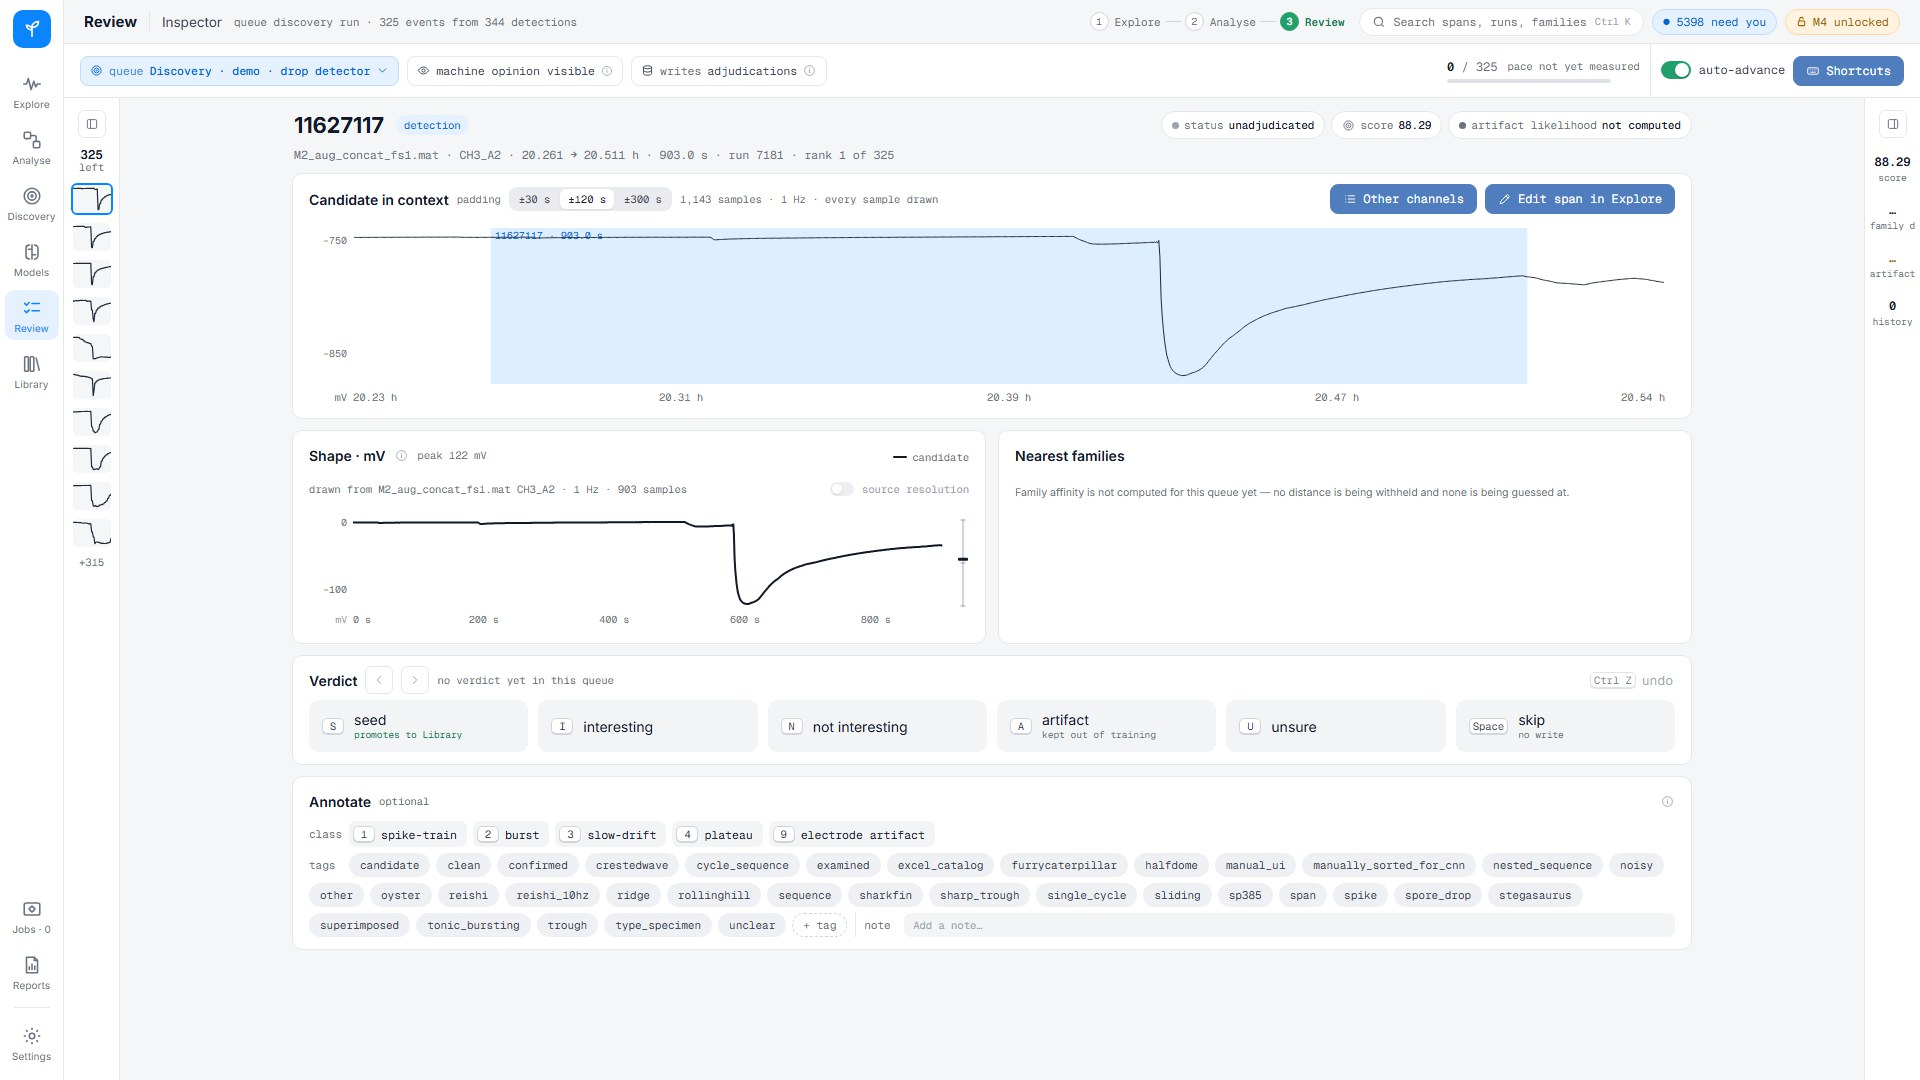
\includegraphics[width=\textwidth]{screens/review_queue.jpg}
\caption{A Review queue in \tool{}: one candidate at a time, the five verdict keys, and machine sections masked in blind queues.}
\label{fig:reviewscreen}
\end{figure}

\begin{instructions}
Add:
\begin{itemize}
  \item the plan said ``seed, uninteresting, or intermediate''; as built, the vocabulary is five fixed words, and no
        sixth word is allowed (Q45);
  \item carried verdicts: a verdict is copied onto matching detections in other runs; copies carry
        \texttt{carried\_from} and are never counted as independent looks;
  \item free human spans live in \texttt{annotations};
  \item blind queues and their masking;
  \item current counts (own looks only, up to 25 Oct): 15,385 human judgements. These are 12,619 annotations
        (including the 11,234 imported 10-minute labels and 1,100 blind showings) and 2,766 own adjudications, of which
        4,151 were given in the tool. 35,073 carried copies are excluded. Against them sit 11.63\,M detections in 7,438
        runs (\src{docs/thesis/numbers_ledger.md}, rows A12--A13).
\end{itemize}
Tests: \src{tests/test_adjudications.py} (lines 116 and 125) and \src{tests/test_surrogate_never_a_detection.py}.

Re-shoot the screenshot after the freeze on 8765, cropped to the card and the keys.
\end{instructions}

\section{Recipes, provenance and the step cache}
\label{sec:provenance}

Every analysis run is expressed as a \emph{recipe}: an ordered list of analysis blocks with their parameters, hashed to give a stable identifier. Every span, score profile and model produced records the recipe hash that generated it. This is what makes a family size, a per-hour recurrence rate or a cross-recording distribution a reportable number rather than a screenshot. It is also what allows a result to be regenerated months later without reconstructing the conditions by hand.

\begin{instructions}
Cover:
\begin{itemize}
  \item \texttt{recipe\_hash()}, a SHA-256 of canonical JSON (\src{Working/recipes.py}), and the 7,518 configs in the
        database;
  \item the step cache, which makes shared prefixes of chains free;
  \item templates (versioned);
  \item exports, as recipes plus reports (HTML, Markdown and figures).
\end{itemize}
The HPC route: \src{Working/hpc/job_export.py} writes \texttt{recipe.json} plus an \texttt{\#SBATCH} script. The cluster
runs \src{Pipelines/run_recipe/run_recipe.py}, and results come back through the import routes. The RQ4b sweep ran 43
jobs per recording this way and matched the local runs exactly, apart from BEADS, which differed by 1--3 spans per
channel (\src{docs/rq_roundA_2/RQ4b-adoption.md}).
\end{instructions}

\section{Controls built into the tool}
\label{sec:toolcontrols}

\begin{instructions}
Cover:
\begin{itemize}
  \item surrogates as a \texttt{Signal}$\rightarrow$\texttt{Signal} block (phase randomisation, block shuffle, AAFT),
        with paired null runs, coverage 2,587 of 2,936 real runs, and the null's recommended cut in seed search;
  \item the cross-channel bins as implemented (\src{Working/cross_channel.py}): artifact is $|$lag$|\le 1$\,s with
        $|r|\ge0.98$; propagation is 1--50\,s with $|r|\ge0.5$; anything else is independent recurrence. Each bin must
        also beat its own random-time null. Bin edges are editable in Settings;
  \item the held-out lock: \src{Working/config.py}, every refusal calling \texttt{held\_out\_locked()}, the switch typed
        by name and audited (tests: \src{tests/test_heldout_lock.py}, \src{tests/test_heldout_switch.py}).
\end{itemize}
\end{instructions}

\section{The motif library}
\label{sec:library}

Motif identity is \textbf{shape-first}. A library entry is an exemplar span, plus the set of spans matched to it, plus the attached evidence for those matches. Cluster identifiers and manual morphology tags attach as many-to-many annotations and are never the primary key.

This choice does two things. It keeps the comparison between cluster labels and manual labels answerable, because neither labelling scheme is privileged in the data model. And it keeps the morphology vocabulary (Appendix~\ref{app:vocab}) a hypothesis under test rather than ground truth. Because identity is shape-first, grouping the library by shape, by cluster or by tag is one selector over one data model rather than three separate implementations.

\begin{figure}[htbp]
\centering
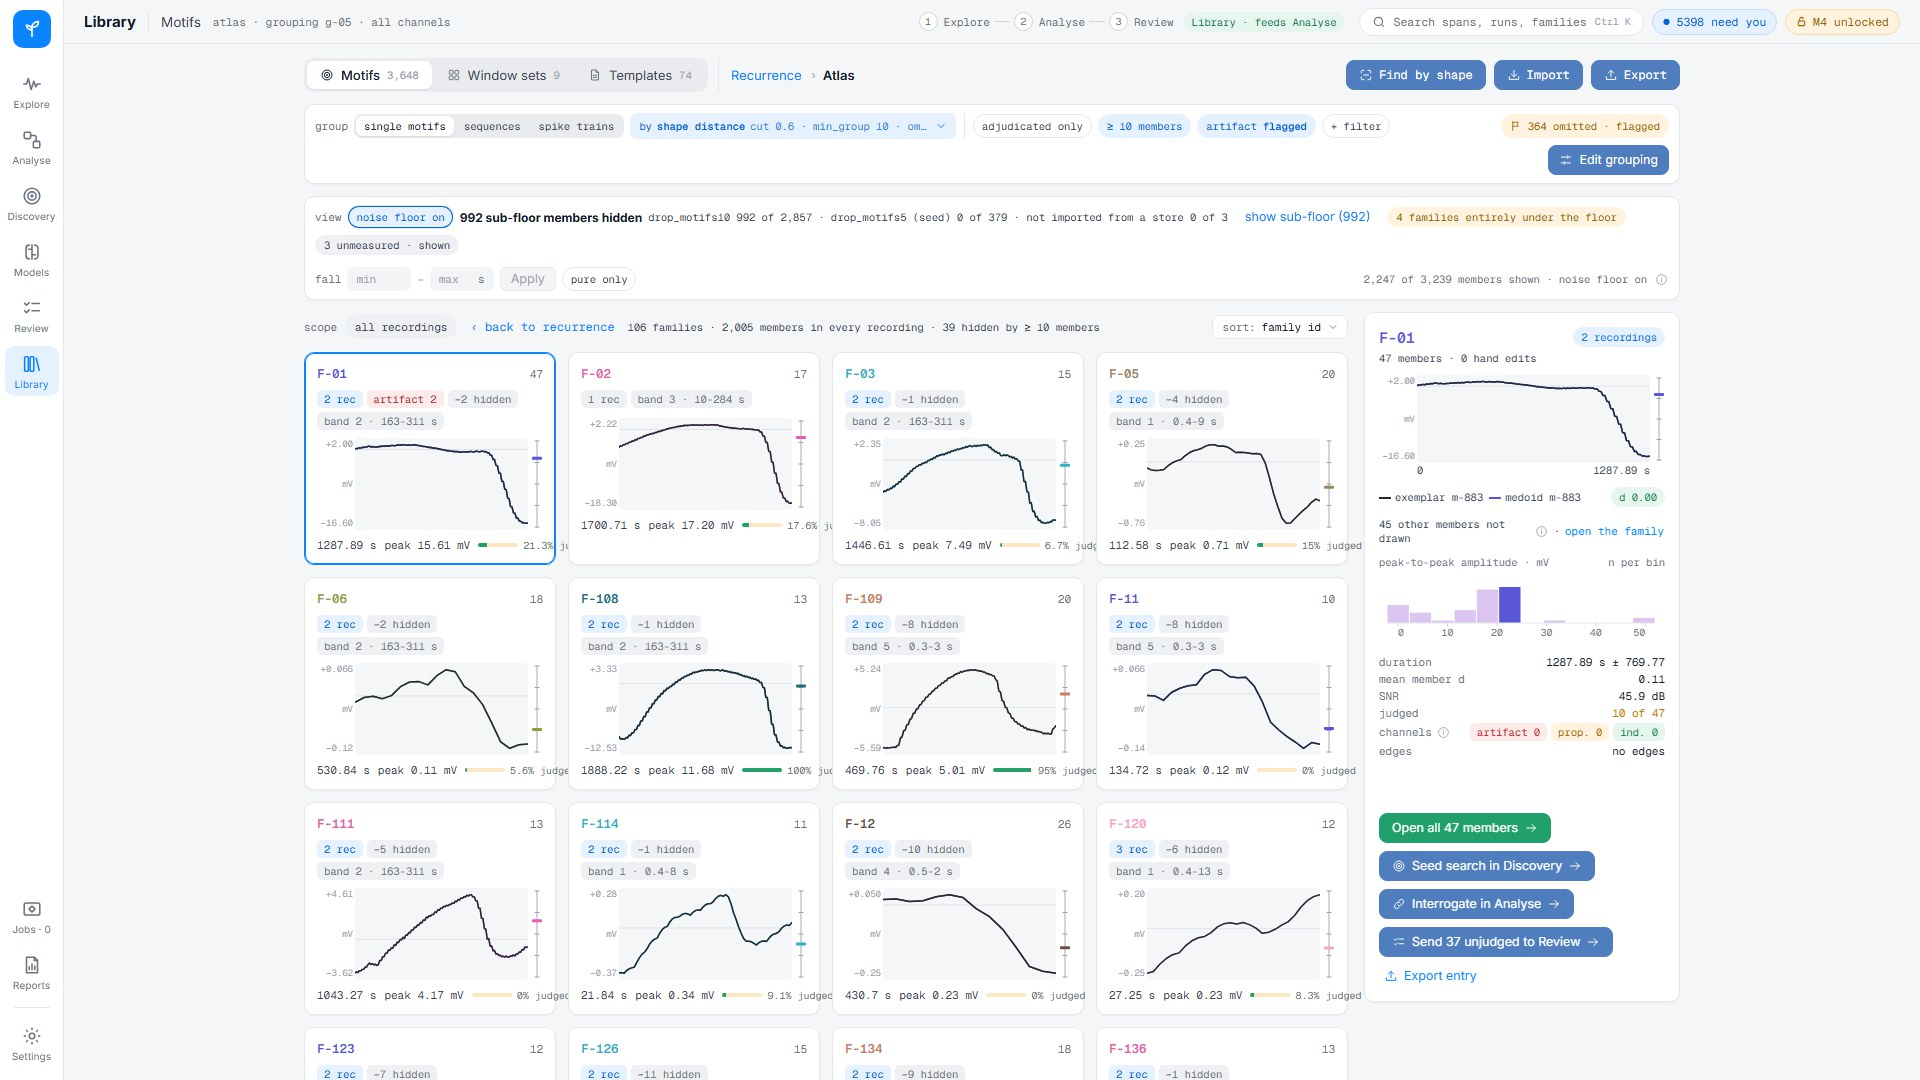
\includegraphics[width=\textwidth]{screens/library_atlas.jpg}
\caption{Library \textrightarrow{} Atlas: a Ward tree of library members cut into shape families (grouping g-05).}
\label{fig:atlasscreen}
\end{figure}

\begin{instructions}
Correct the plan's claim that similarity edges are persisted. The schema exists: \texttt{motif\_edge} stores the
distance function, threshold, value, recipe hash, lag, waveform correlation and bin. But the live database has 0 edges.
Family membership is persisted through groupings instead.

State the grouping you use throughout (Round 3 decision), and the fragment audit: 67\,\% of g-05's members are
overlapping 2-second pieces of one 20-minute reishi recording, and they dominate 115 of its 149 families. Your accepted
set is 197 members, which are 142 distinct events
(\src{docs/rq_roundA_2/findings/library-fragments-and-duplicates.md}).
\end{instructions}

\section{The workflow through the pages}
\label{sec:workflow}

\begin{instructions}
New, about one page with figures. Show the path one motif takes through the pages: Explore $\rightarrow$ Analyse
$\rightarrow$ Discovery $\rightarrow$ Review $\rightarrow$ Library, with Models branching off the Library. The poster's stylised panels are cut (5 Nov); use the
re-shot screenshots (Figure~\ref{fig:pages}), following motif 458 (M2\_aug CH1\_A1 at 316.2\,h, family F-80) where
possible. There are 50 pages in all:
34 main pages and 16 settings pages (\src{webui/client/src/shell/pages.ts}).

Then name the three workflows the demonstration walked:
\begin{itemize}
  \item W1, characterise a spike train: \texttt{spike\_event\_features}; 85 spans covering 88 of about 90 spikes after
        two parameter changes;
  \item W2, build a detector on a 4-hour span and apply it to 5 channels $\times$ 721\,h: 6 drops on the span, 365 at
        scale, against a 20-draw null;
  \item W3, grow a family from one example: F-30, a seed search, 155 matches kept under the null's cut.
\end{itemize}
Source: \src{docs/DEMO_DAY.md}.
\end{instructions}

\begin{figure}[htbp]
\centering
\figplaceholder{6cm}{Figures 4.4 (T1, screenshots, wave 3): the pages re-shot in one pass, light theme, one viewport ---
Explore, Analyse, Discovery, Review, Library and Models --- following one motif where possible.}
\caption{The pages of \tool{}.}
\label{fig:pages}
\end{figure}

\begin{figure}[htbp]
\centering
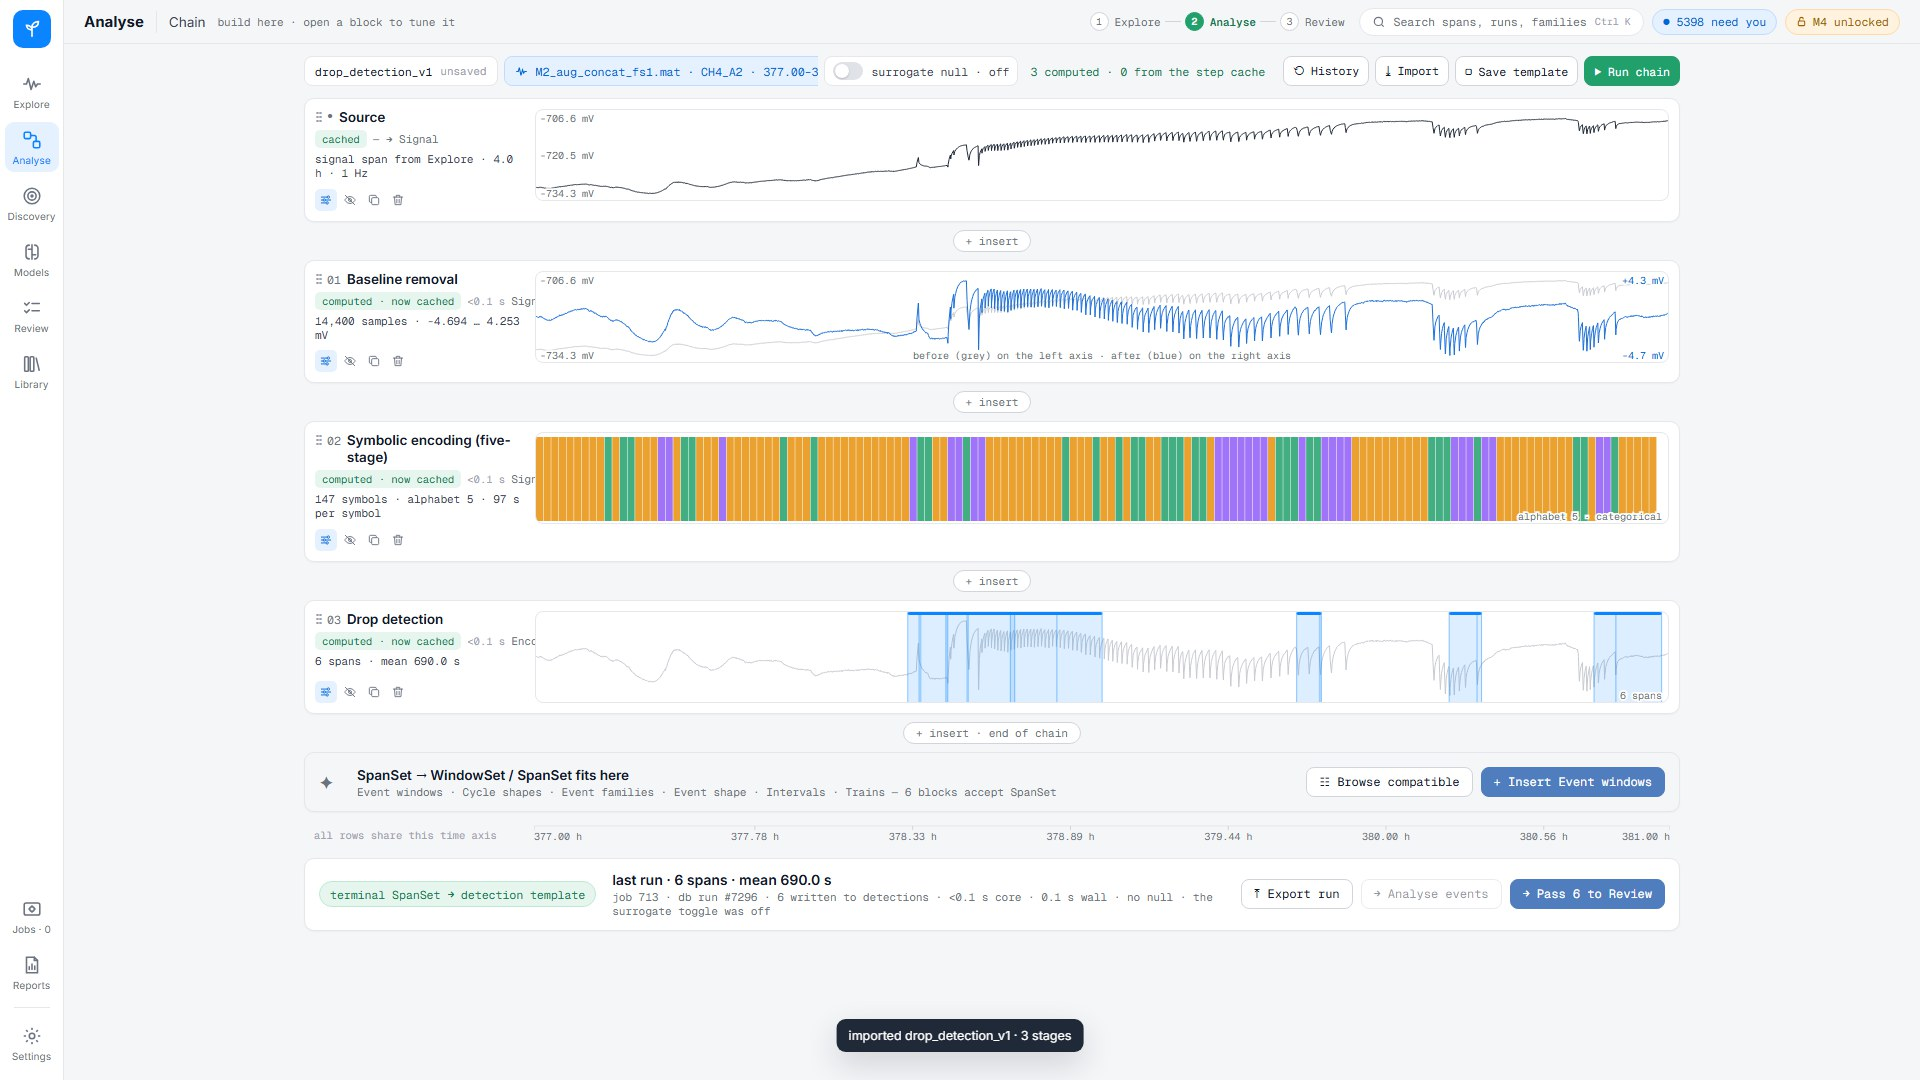
\includegraphics[width=\textwidth]{screens/analyse_drop_detector.jpg}
\caption{Analyse: a chain built on a 4-hour span (drop detector, 6 drops), before it is saved as a template and applied to 721 hours.}
\label{fig:analysescreen}
\end{figure}

\section{How MycoWave was built}
\label{sec:buildmethod}

\begin{instructions}
New, about 1.5 pages; you asked for this section in Q6. Describe the method adapted from Matt Pocock's agent skills
\cite{pocockskills}, as a pipeline:
\begin{enumerate}
  \item \textbf{grilling}: adversarial questioning of a design until every branch is settled by you;
  \item \textbf{to-spec}: the settled decisions written as a product requirements document. \src{docs/PIPELINE_PRD.md},
        613 lines: Part 1 (tickets T01--T49) settled through a goals grilling and a design grilling; Part 2, the
        Usability Wave (T50+), settled 27 Aug;
  \item \textbf{to-tickets}: decomposition into vertical slices, each cutting through every layer and independently
        testable. 70 tickets (\src{docs/tickets/}) with a dependency graph, mutexes and a model/size table;
  \item \textbf{test-first, one agent per ticket}: the first commit of a ticket touches only \texttt{tests/} and must
        fail; the orchestrator checks out that commit and confirms it is red before implementation is allowed;
  \item \textbf{gates}: red proof, the suite, scope (out-of-list files reported to the reviewer), review, and file
        overlap between parallel tickets.
\end{enumerate}

Then the two generations.

The orchestrator (\src{orchestrator/}, \src{docs/ORCHESTRATOR_SPEC.md}):
\begin{itemize}
  \item deterministic standard-library code, about 6,900 lines and 316 tests by 19 Aug; no model makes scheduling or
        merge decisions;
  \item each ticket ran as \texttt{claude -p} in its own git worktree, with permission prompts disabled, which the
        worktree isolation makes acceptable;
  \item merges went to \texttt{integration/run-*} branches, never \texttt{main}: 12 runs, 55 merged tickets;
  \item Claude Haiku, Sonnet and Opus until 25 Aug; then DeepSeek V4 flash and pro for 50 of the 55 merges, with review
        and fix rounds on Claude. This built the first, Panel-based version and its core structures.
\end{itemize}

The Panel interface was retired on 21 Sep (tag \texttt{archive/panel-ui}). Why: a surface that constructs has not
necessarily painted. The React rewrite (ADR 0001) was then built in Claude Code sessions as waves of prompts:
\begin{itemize}
  \item wiring 6, blocks 26, fixup 51, changes 20, quality 12;
  \item implementer agents with separate critic agents (28 critic reports, 16 fix rounds; \src{docs/prompts/quality/critic.md});
  \item at most three implementers at once, because six made every timing meaningless;
  \item the per-merge UI gate: type-check, build, the change's own tests, and the smoke units it touches.
\end{itemize}

Numbers: 1,779 commits, the first on 14 Apr 2026; 1,134 of them in October; 368 commits touch only \texttt{tests/};
1,574 carry an AI co-author line. Your role: spec author, decision maker, reviewer and tester.

An honest note on cost: the method trades human typing for human review. Several critic catches were real regressions
the implementers missed (\src{docs/prompts/quality/REVIEW.md}).
\end{instructions}

\section{Evaluation of the tool}
\label{sec:tooleval}
\label{sec:pipelineeval}

\begin{instructions}
About 1.5 pages. The plan said the tool is evaluated on generalisation and on nothing else. Keep generalisation as the
headline: the held-out exam, reported in Chapter~\ref{ch:rq3} with its exposure record in
Chapter~\ref{ch:method}. Add the assertions that are tested:
\begin{itemize}
  \item reproducibility: the same recipe hash gives the same output
        (\src{tests/test_recipes.py}, lines 39--90; \src{tests/test_execution.py}, line 71: an identical recipe reuses
        the prior run);
  \item the human/machine separation (tests above);
  \item a surrogate is never counted as a detection.
\end{itemize}
Scale reached: 7,438 runs; 11.63\,M detections; RQ4b sweeps of 43 jobs per recording on 6 recordings; 5,567 tests
passing in the 21 Oct daily run; an 832-screenshot smoke walk over 64 page specs.

Problems met and how they were answered (the marksheet asks for this):
\begin{itemize}
  \item the 21 Sep data loss, when \texttt{git worktree remove} followed a directory junction. Recovery: the database
        from a sandbox copy, the channels re-derived; rule: unlink junctions first;
  \item Dehshibi's paper and code disagree; the authors' code was followed (Q33);
  \item M2\_concat and M2\_aug turned out to be different data;
  \item null draws overwrote the real matrix profile (fixed);
  \item the drop detector assumed volts (fixed 15 Oct);
  \item seed-search pile-up: 20 duplicate jobs, leading to the HPC route;
  \item the Library fragment audit;
  \item CNN training provenance was never recorded;
  \item the held-out exposure.
\end{itemize}

Alternatives considered and rejected:
\begin{itemize}
  \item Panel vs React, from prototypes (ADR 0001);
  \item a node canvas vs a linear chain ribbon;
  \item an ORM vs plain SQL;
  \item one concatenated channel vs per-channel analysis;
  \item a whole-signal matrix profile (40--260\,h) vs seeded search (seconds);
  \item CNN vs random features vs a hand-crafted-feature forest.
\end{itemize}
\end{instructions}

\section{Scope as built}
\label{sec:scope}

The thesis plan recorded a set of deliberate exclusions so that the thesis would not be read as claiming them. Table~\ref{tab:scope} records what became of each.

\begin{table}[htbp]
\caption{Planned scope exclusions (August 2026) against the software as built (October 2026).}
\label{tab:scope}
\small
\begin{tabularx}{\textwidth}{p{4.2cm} p{2.2cm} X}
\toprule
\textbf{Planned exclusion} & \textbf{Status} & \textbf{As built}\\
\midrule
Multivariate analysis & partly built & Cross-channel lag, correlation and three-bin classification, and an Explore cross-channel page; no multivariate models.\\
Data import robustness & built & Registration with checks, excerpt detection, unit and rate inference, a Settings import page.\\
An open plugin architecture & not built & The block contract makes a new block easy to add; there is no third-party registry.\\
A drag-and-drop node canvas & not built & Chains are a linear ribbon of typed blocks.\\
Rendered report generation & built & HTML, Markdown and figure reports per run.\\
Cross-domain corpora & not built & No non-fungal control; cross-species fungal data was added instead.\\
A supported software release & partly & A 342-page user manual; not packaged or supported.\\
Biological interpretation & excluded & Unchanged (Section~\ref{sec:position}).\\
\bottomrule
\end{tabularx}
\end{table}
